\chapter{Installer le logiciel}

\section{Consultez la documentation du framework !}

Le logiciel a été conçu à partir du framework \textit{Prototypephp}. La documentation associée \cite{pphp-doc} récapitule l'ensemble des informations nécessaires pour réaliser l'installation générale (configuration du serveur, définition des droits d'accès, etc.).

De nombreuses passages ont été repris ici, mais il n'est pas inutile de se référer au document d'origine. 

\section{Installation automatique}
Le logiciel est livré avec un script qui installe automatiquement les paquets nécessaires, télécharge le code de l'application depuis Github, crée la base de données et prépare la configuration du serveur web Apache.

L'installateur est conçu pour fonctionner avec une distribution Debian ou Ubuntu (version LTS).

\subsection{Mode opératoire}
\begin{itemize}
	\item installez une distribution Linux (préférentiellement, la dernière Debian stable) ;
	\item connectez-vous en mode \textit{root} ;
	\item téléchargez le script d'installation : \href{https://github.com/Irstea/collec/raw/master/install/deploy_new_instance.sh}{deploy\_new\_instance.sh} avec la commande :
	\begin{lstlisting}
	wget https://github.com/Irstea/collec/raw/master/install/deploy_new_instance.sh
	chmod +x deploy_new_instance.sh
	\end{lstlisting}
	\item exécutez le script, qui va réaliser l'ensemble des opérations automatisables ;
	\item éditez ensuite le fichier /etc/apache2/sites-available/collec-science.conf, pour positionner correctement le dns de votre application et indiquer les informations liées au certificat https (clé privée, certificat, autorité de certification) ;
	\item activez le site, puis rechargez Apache :
	\begin{lstlisting}
	a2ensite collec-science
	systemctl reload apache2
	\end{lstlisting}
\end{itemize}

\section{Installation manuelle}
\subsection{Configurer le serveur}

L'application est conçue pour fonctionner à partir d'une adresse unique de type : {\NoAutoSpacing\textit{https://monsite.com}}. Le chiffrement est obligatoire (protocole https). Il n'est pas possible d'installer l'application dans un sous-dossier, par exemple : \linebreak{\NoAutoSpacing \textit{https://monsite.com/collec-science}} ne fonctionnera pas.


\subsection{Configurer Apache}
Les modules suivants doivent être activés :
\begin{lstlisting}
a2enmod ssl
a2enmod headers
a2enmod rewrite
\end{lstlisting}

\subsection{Modules PHP nécessaires}
PHP doit être en version 7.2 au minimum. Il est préférable d'installer PHP depuis le site de PHP plutôt que d'utiliser les paquets fournis par la distribution.

Modules complémentaires nécessaires :
\begin{itemize}
\item \textit{php-mbstring}
\item \textit{php-pgsql}
\item \textit{php7.x-xml} 
\item \textit{php-xdebug} pour les phases de mise au point
\item \textit{php-curl} pour l'identification via un serveur CAS.
\end{itemize}
La génération des étiquettes nécessite les paquetages suivants :
\begin{itemize}
\item \textit{php-gd} 
\item \textit{fop} (qui inclut des bibliothèques java)
\end{itemize}

Le stockage et l'affichage des photos nécessite :
\begin{itemize}
\item \textit{php-imagick}
\end{itemize}

\subsection{Installer et configurer php}
Voici un extrait du script d'installation automatique qui permet d'installer PHP :
\begin{lstlisting}
PHPVER=7.3
PHPINIFILE="/etc/php/$PHPVER/apache2/php.ini"
apt -y install lsb-release apt-transport-https ca-certificates
DISTRIBCODE=`lsb_release -sc`
DISTRIBNAME=`lsb_release -si`
if [ $DISTRIBNAME == 'Ubuntu' ]
then
apt-get install software-properties-common
add-apt-repository -y ppa:ondrej/php
add-apt-repository -y ppa:ondrej/apache2
elif [ $DISTRIBNAME == 'Debian' ]
then
wget -qO https://packages.sury.org/php/apt.gpg | apt-key add -
echo "deb https://packages.sury.org/php/ $DISTRIBCODE main" | tee /etc/apt/sources.list.d/php.list
fi
apt-get update
apt-get -y install unzip apache2 libapache2-mod-evasive libapache2-mod-php$PHPVER php$PHPVER php$PHPVER-ldap php$PHPVER-pgsql php$PHPVER-mbstring php$PHPVER-xml php$PHPVER-zip php$PHPVER-imagick php$PHPVER-gd
\end{lstlisting}

De plus, après installation, la configuration du fichier php.ini doit être modifiée pour garantir un fonctionnement optimal du logiciel :
\begin{lstlisting}
# adjust php.ini values
upload_max_filesize="=100M"
post_max_size="=50M"
max_execution_time="=120"
max_input_time="=240"
memory_limit="=1024M"
max_input_vars="10000"
for key in upload_max_filesize post_max_size max_execution_time max_input_time memory_limit
do
 sed -i "s/^\($key\).*/\1 $(eval echo \${$key})/" $PHPINIFILE
done
sed -i "s/; max_input_vars = .*/max_input_vars=$max_input_vars/" $PHPINIFILE
\end{lstlisting}

Enfin, l'outil de gestion des images a besoin d'être reconfiguré, pour autoriser la manipulation des images :
\begin{lstlisting}
# adjust imagick policy
sed -e "s/  <policy domain=\"coder\" rights=\"none\" pattern=\"PDF\" \/>/  <policy domain=\"coder\" rights=\"read|write\" pattern=\"PDF\" \/>/" /etc/ImageMagick-6/policy.xml > /tmp/policy.xml
cp /tmp/policy.xml /etc/ImageMagick-6/
\end{lstlisting}

\subsection{Configurer l'antivirus}
Les pièces téléchargées peuvent être analysées avec l'antivirus CLAMAV \cite{clamav}. Dans un premier temps, Clamav doit être installé. Le plus simple est d'utiliser les paquetages de la distribution.

Suivez les instructions du document \cite{clamavarchlinux} pour l'installation et la vérification du bon fonctionnement.

Par défaut, le script d'installation automatique n'installe pas l'antivirus. Si vous souhaitez activer cette fonctionnalité, vous devrez la configurer vous-même.

\subsection{Configurer l'hôte virtuel et SSL}
L'application ne fonctionne qu'en mode SSL, les cookies de session n'étant pas transmis sur des liens non chiffrés. Voici un exemple de configuration à insérer dans le fichier \textit{/etc/apache2/sites-available/default-ssl}
\begin{lstlisting}
    <Directory /var/www/html>
        Options FollowSymLinks MultiViews
        AllowOverride all
        Order allow,deny
        allow from all
    </Directory>
SSLProtocol             all -SSLv3
SSLCipherSuite          ECDHE-ECDSA-CHACHA20-POLY1305:ECDHE-RSA-CHACHA20-POLY1305:ECDHE-ECDSA-AES128-GCM-SHA256:ECDHE-RSA-AES128-GCM-SHA256:ECDHE-ECDSA-AES256-GCM-SHA384:ECDHE-RSA-AES256-GCM-SHA384:DHE-RSA-AES128-GCM-SHA256:DHE-RSA-AES256-GCM-SHA384:ECDHE-ECDSA-AES128-SHA256:ECDHE-RSA-AES128-SHA256:ECDHE-ECDSA-AES128-SHA:ECDHE-RSA-AES256-SHA384:ECDHE-RSA-AES128-SHA:ECDHE-ECDSA-AES256-SHA384:ECDHE-ECDSA-AES256-SHA:ECDHE-RSA-AES256-SHA:DHE-RSA-AES128-SHA256:DHE-RSA-AES128-SHA:DHE-RSA-AES256-SHA256:DHE-RSA-AES256-SHA:ECDHE-ECDSA-DES-CBC3-SHA:ECDHE-RSA-DES-CBC3-SHA:EDH-RSA-DES-CBC3-SHA:AES128-GCM-SHA256:AES256-GCM-SHA384:AES128-SHA256:AES256-SHA256:AES128-SHA:AES256-SHA:DES-CBC3-SHA:!DSS
SSLHonorCipherOrder     on
SSLCompression          off
SSLSessionTickets       off

\end{lstlisting}

(attention : pas d'espace entre \textit{Order allow} et la virgule).

La chaîne \textit{SSLCipherSuite} est celle qui fonctionne avec Apache 2.4.24 et openssl 1.1.0f, et est issue du configurateur mis à disposition par la fondation Mozilla \cite{mozillagenerator}. 
Vous pouvez également consulté le document édité par l'ANSSI \cite{tls}. 

Activez ensuite le mode SSL dans Apache :
\begin{lstlisting}
a2ensite default-ssl
service apache2 restart
\end{lstlisting}

\subsection{Configurer Apache pour l'identification à partir d'une fédération}
\label{mellon}
À partir de la version 2.4.0, Collec-Science permet d'identifier les utilisateurs à partir d'une fédération d'identités, comme la fédération française RENATER ou EDUGAIN (la fédération internationale des instituts universitaires et de recherche).

Cette identification n'est possible que pour les applications accessibles depuis Internet, et s'appuie sur l'utilisation d'un module Apache dédié : \textit{Mellon}. Elle nécessite également de récupérer les informations techniques liées à la fédération, et d'enregistrer l'application chez le fournisseur de l'identification.

\subsubsection{Installation du module Mellon}
\begin{lstlisting}
apt-get install libapache2-mod-auth-mellon
\end{lstlisting}

Si le paquet libapache2-mod-auth-mellon n'est pas disponible (cas rencontré avec une distribution Debian strech), vous devrez récupérer et installer les paquets suivants (dans l'ordre) :
\begin{itemize}
	\item libxmlsec1
	\item libxmlsec1-openssl
	\item liblasso3
	\item libapache2-mod-auth-mellon
\end{itemize}

Vous devrez également récupérer le fichier xml de votre \textit{provider}, ainsi que son certificat.

\subsubsection{Génération des fichiers de configuration de l'application}
Un certificat (et sa clé privée), un fichier xml doivent être générés pour l'application. Un script est disponible dans les distributions Debian. Il est également fourni dans l'application, dans le dossier install/apache2 (\textit{create\_metadata.sh}).

Pour générer les fichiers (remplacez \textit{collec-science.com} par vos propres valeurs) : 
\begin{lstlisting}
cd /etc/apache2
mkdir mellon
cd mellon
/var/www/html/collec-science/collec/install/apache2/create_metadata.sh https://collec-science.com https://collec-science.com/mellon
\end{lstlisting}

Le certificat (fichier .cert) et le fichier xml doivent être transmis au \textit{provider}, pour qu'il les intègre dans sa plate-forme.

Vous devez également récupérer du \textit{provider} sa clé publique et son certificat d'autorité racine, à mettre dans le dossier \textit{mellon}. Il doit également vous fournir un fichier xml qui contient les adresses de toutes les entités participant à la fédération.

\subsubsection{Configurer le site virtuel}

Recopiez le fichier install/apache2/collec-science-mellon.conf dans le dossier /etc/apache2/sites-available, à la place du fichier collec-science.conf
Éditez le fichier, et remplacez toutes les chaînes \textit{collec.mysociety.com} par votre DNS. Vérifiez également les certificats utilisés.

Par rapport au fichier classique, le fichier \textit{collec-science-mellon.conf} contient, dans la section \textit{<VirtualHost *443>}, les commandes suivantes :
\begin{lstlisting}
    # Configuration Mellon for Renater
    <location />
    AuthType Mellon
    MellonEnable "auth"
    MellonSecureCookie On
    MellonUser MAIL
    MellonMergeEnvVars On
    MellonSubjectConfirmationDataAddressCheck Off
    MellonSPPrivateKeyFile /etc/apache2/mellon/https_collec.mysociety.com.key
    MellonSPCertFile /etc/apache2/mellon/https_collec.mysociety.com.cert
    MellonSPentityId "https://collec.mysociety.com"
    MellonSPMetadataFile "/etc/apache2/mellon/https_collec.mysociety.com.xml"
    MellonIdPMetadataFile "/etc/apache2/mellon/main-idps-renater-metadata.xml"
    MellonIdPPublicKeyFile "/etc/apache2/mellon/renater-metadata-signing-cert-2016.pem"
    MellonIdPCAFile "/etc/apache2/mellon/renater-metadata-signing-cert-2016.pem"
    MellonProbeDiscoveryTimeout 1
    MellonSetEnv "MAIL" "urn:oid:0.9.2342.19200300.100.1.3"
    MellonSetEnv "GIVENNAME" "urn:oid:2.5.4.42"
    MellonEndpointPath /mellon
    MellonSetEnvNoPrefix REMOTE_USER NAME_ID
    MellonDiscoveryURL "https://discovery.renater.fr/renater/WAYF"
    </location>
\end{lstlisting}

Les rubriques \textit{MellonIdP*} doivent être adaptées aux fichiers fournis par votre provider.

Une fois la configuration effectuée, redémarrez le serveur Apache :
\begin{lstlisting}
systemctl restart apache2
\end{lstlisting}

\subsubsection{Configuration du logiciel}
Modifiez le fichier \textit{param/param.inc.php}, avec les informations suivantes :

\begin{lstlisting}
$ident_type = "HEADER";
$MAIL_enabled = 1;
\end{lstlisting}

\subsubsection{Enregistrer le site dans la fédération Renater}

Pour les établissements français affiliés à la fédération Renater, vous pouvez enregistrer directement votre application dans celle-ci. Des validations seront réalisées par les contacts de la fédération dans votre établissement.

Pour réaliser l'enregistrement :
\begin{itemize}
	\item Connectez-vous au site \href{https://federation.renater.fr/registry}{https://federation.renater.fr/registry}
	\item cliquez sur \textit{Ajouter un fournisseur de services}
	\item  dans l'onglet \textit{Description}, renseignez les champs demandés, avec notamment :
	\begin{itemize}
		\item URL du service : https://collec.mysociety.com (votre DNS)
	\end{itemize}
	\item  dans l'onglet \textit{Contacts}, ne vous déclarez pas conforme au cadre de sécurité SIRTFI, sauf si vous savez ce que c'est (il y a des contraintes organisationnelles fortes pour être conforme)
	\item dans l'onglet \textit{Attributs demandés}, demandez les attributs :
	\begin{itemize}
		\item email : identification des utilisateurs (obligatoire)
		\item commonName : affichage du nom des utilisateurs (obligatoire)
	\end{itemize}
	\item dans l'onglet \textit{Informations techniques}, indiquez l'adresse suivante pour récupérer les données de configuration :
	\begin{itemize}
		\item URL de vos métadonnées : https://collec.mysociety.com/mellon/metadata
	\end{itemize}
\end{itemize}

Une fois le dossier validé, vous devrez attendre le retour de votre correspondant Renater dans votre établissement, qui doit valider votre demande.

Une fois cette première demande réalisée, vous devrez vous reconnecter au site de la fédération (\href{https://federation.renater.fr/registry}{https://federation.renater.fr/registry}), et activer le rattachement à la fédération choisie (onglet \textit{Rattachement à une fédération}). Deux fichiers seront à récupérer (commande wget dans le dossier /etc/apache2/mellon) pour récupérer d'une part le certificat, et d'autre part le fichier XML contenant l'ensemble des fournisseurs attachés à la fédération.

Ce rattachement doit également être validé par votre correspondant Renater.

\underline{Attention :} une fois le rattachement validé, vous devrez attendre 24 heures pour que votre application soit disponible auprès de l'ensemble des membres de la fédération, et donc pouvoir vous connecter à l'application. Dans le cas contraire, vous obtiendrez des messages d'erreur.
 

\subsection{Configurer le dossier d'installation}

Le principe général est que le dossier contenant l'application contient, dans son nom, le numero de version (collec-2.0 par exemple), et un lien virtuel (collec) pointe vers celui-ci. C'est le lien qui est la cible de l'adresse web : ainsi, à chaque nouvelle version, il suffit de mettre à jour le code de l'application et de faire pointer le lien vers le nouveau dossier pour que celle-ci soit opérationnelle.

Depuis la version 2.0, des scripts sont fournis pour réaliser automatiquement les mises à jour (dans le cas d'installations mono-instances).

\subsubsection{Cas général : une seule instance hébergée dans le serveur}

Utilisez le script fourni, qui créera automatiquement les dossiers nécessaires. 


\subsubsection{Cas particulier : faire cohabiter plusieurs instances avec le même code}
\label{dnsmultiple}
Il est possible d'utiliser le même code applicatif pour alimenter des bases de données différentes (ou des données stockées dans des schémas différents). Cette fonctionnalité est basée sur l'attribution d'entrées DNS différentes. 

Le mécanisme est décrit dans la figure \ref{dnsmultipleschema} \textit{\nameref{dnsmultipleschema}}, page \pageref{dnsmultipleschema}.

\begin{figure}[H]
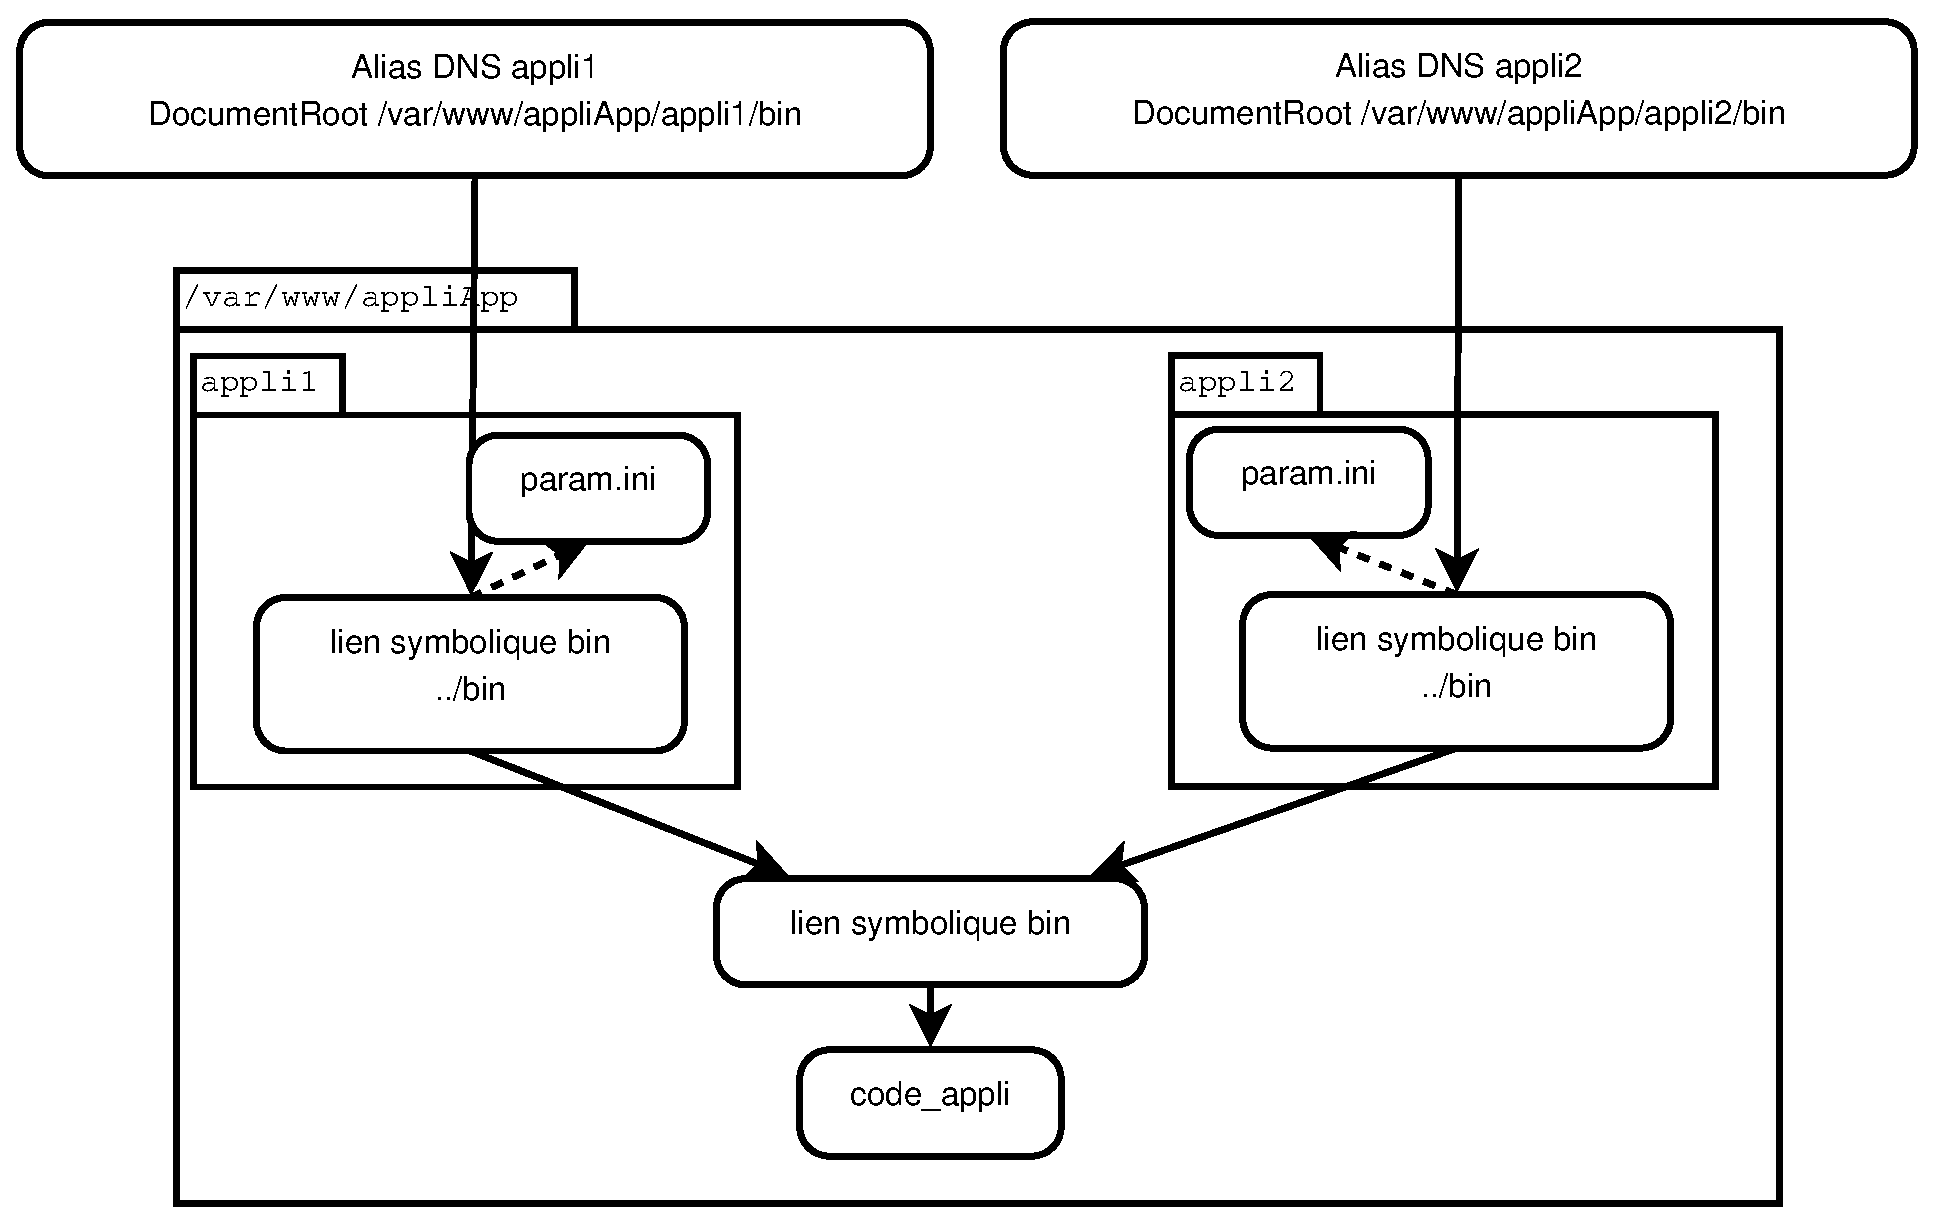
\includegraphics[width=\linewidth]{images/dnsmultiple}
\caption{\label{dnsmultipleschema}Schéma général d’implémentation pour utiliser le même code avec des noms d’application et des jeux de données différents}
\end{figure}

Dans le paramétrage de l’alias DNS (en principe, dans \textit{/etc/apache2/sites-available}), l’application pointe vers le dossier \textit{/var/www/appliApp/appli1/bin}. \textit{/var/www} correspond à la racine du site web, \textit{appliApp} au dossier racine de l’application, \textit{appli1} au dossier spécifique de l’alias DNS. Ce dossier \textit{appli1} ne contient que deux fichiers : \textit{param.ini}, qui contient les paramètres spécifiques, et \textit{bin}, qui est un lien symbolique vers le dossier \textit{../bin}.

Le dossier \textit{../bin} (donc, dans\textit{ /var/www/appliApp}) est lui aussi un alias qui pointe vers le code réel de l’application, ici \textit{code\_appli}. Le fichier \textit{param.inc.php} doit contenir les commandes suivantes pour que le fichier \textit{param.ini} soit correctement chargé selon le contexte :
\begin{lstlisting}
$chemin = substr($_SERVER["DOCUMENT_ROOT"],0, strpos($_SERVER["DOCUMENT_ROOT"],"/bin"));
$paramIniFile = "$chemin/param.ini";
\end{lstlisting}

Le fichier \textit{param.ini} sera cherché dans le dossier parent du code de l’application, c’est à dire soit dans \textit{appli1}, soit dans \textit{appli2} dans cet exemple. Il suffit qu’il contienne les paramètres adéquats pour rendre l’application utilisable dans des contextes différents à partir du même code initial.

Le fichier \textit{param.ini} est le dernier qui est traité par l'application pour récupérer les paramètres. Ceux-ci sont lus dans l'ordre suivant :

\textbf{param/param.default.inc.php $\rightarrow$ param/param.inc.php $\rightarrow$ ../param.ini}

\textit{param.ini} contiendra les entrées spécifiques liées au DNS utilisé pour accéder à l'application, en principe tout ou partie de celles-ci :
\begin{lstlisting}
APPLI_titre="Gestion des collections d'EABX"
BDD_schema=col, public, gacl
BDD_login=compte_de_connexion
BDD_passwd=mot_de_passe_de_connexion
BDD_dsn=pgsql:host=serveur;dbname=base_de_donnees;sslmode=require
GACL_aco=col
APPLI_code=proto
\end{lstlisting}

Si un libellé contient une apostrophe, la chaîne doit être insérée dans des guillemets doubles, comme ici pour la variable \textit{APPLI\_titre}.


\subsection{Droits à attribuer au serveur web}
\label{droitsApache}
Le serveur web doit pouvoir accéder en lecture à l'ensemble des fichiers de l'application, et en écriture à deux dossiers :
\begin{itemize}
\item \textit{display/templates\_c} : fichier utilisé par Smarty pour compiler les modèles de documents HTML ;
\item \textit{temp} : dossier de génération des images et des fichiers temporaires.
\end{itemize}

Deux scripts sont fournis pour attribuer les droits : 
\begin{itemize}
\item \textbf{install/apache2/upgrade\_rights.sh} : positionne les droits en utilisant les droits standards Linux (owner, group)
\item \textbf{install/apache2/upgrade\_rights\_with\_acl.sh} : positionne les droits à partir des ACL.
\end{itemize}

Les scripts doivent être lancés ainsi :
\begin{lstlisting}
collec-2.0/install/apache2/upgrade_rights.sh collec-2.0
\end{lstlisting}
ou 
\begin{lstlisting}
collec-2.0/install/apache2/upgrade_rights_with_acl.sh collec-2.0
\end{lstlisting}


\section{Configurer l'application}

L'application est configurable par l'intermédiaire de trois fichiers :

\textbf{param/param.default.inc.php $\rightarrow$ param/param.inc.php $\rightarrow$ ../param.ini}

Le premier fichier contient les paramètres par défaut. Il est systématiquement fourni à chaque nouvelle version de l'application.

Le second est spécifique de l'implémentation. Il comprend notamment les informations liées à la connexion à la base de données, à la méthode d'identification, ou à la recherche des attributs dans l'annuaire LDAP. 

le troisième est destiné à offrir la possibilité d'accéder, à partir du même code applicatif, à plusieurs bases de données différentes (\textit{cf.} \ref{dnsmultiple} \textit{\nameref{dnsmultiple}}, page \pageref{dnsmultiple}).

Voici les principaux paramètres utilisés :

\subsection{Connexion à la base de données}

Dans la pratique, deux connexions sont nécessaires : l'une pour accéder à la base des droits, l'autre aux données proprement dites. Voici les paramètres à définir :

\begin{longtable}{|p{4cm}|p{11cm}|}
\hline
\textbf{Variable} & \textbf{Signification} \\
\hline
\endhead
BDD\_login & compte de connexion à la base de données \\
\hline
BDD\_passwd & mot de passe associé\\
\hline
BDD\_dsn & adresse de la base de données sous forme normalisée\\
\hline
BDD\_schema & schéma utilisé (plusieurs schémas peuvent être décrits, en les séparant par une virgule - fonctionnement propre à Postgresql)\\
\hline
GACL\_dblogin & compte de connexion à la base de données des droits\\
\hline
GACL\_dbpasswd & mot de passe associé\\
\hline
GACL\_dsn & adresse normalisée \\
\hline
GACL\_schema & schéma utilisé\\
\hline
GACL\_aco & nom du code de l'application utilisé dans la gestion des droits\\
\hline
\caption{Variables utilisées pour paramétrer les connexions}
\end{longtable}

\subsection{Identification des utilisateurs}

\begin{longtable}{|p{6cm}|p{10cm}|}
\hline
\textbf{Variable} & \textbf{Signification} \\
\hline
\endhead
ident\_type & Type d'identification supporté :
\begin{itemize}
	\item BDD : uniquement en base de données
	\item LDAP : uniquement à partir d'un annuaire LDAP
	\item LDAP-BDD : test de connexion d'abord auprès de l'annuaire LDAP, puis en base de données en cas d'échec
	\item CAS : identification auprès d'un serveur CAS (Common Access Service)
	\item HEADER : identification auprès d'une fédération d'identités, comme EDUGAIN. Nécessite un paramétrage particulier du serveur Apache2 (\textit{cf.} \ref{mellon})
\end{itemize}
\\
\hline
CAS\_plugin & Nom du plugin utilisé pour une connexion CAS \\
\hline
CAS\_address & Adresse du serveur CAS, sous la forme : \textit{nomserveur.societe.com/cas} (sans préfixer avec https://)\\
\hline
CAS\_port = 443 & port utilisé pour atteindre le serveur CAS (port https)\\
\hline
CAS\_debug = false & true ou false, pour activer ou non l'enregistrement des fonctions de débogage. À positionner systématiquement à \textit{false} en production \\
\hline
CAS\_CApath = "" & Chemin d'accès au certificat de l'autorité de certification qui correspond au certificat fourni par le serveur CAS (connexion https). Si la chaîne est vide, le certificat n'est pas vérifié. Le chemin doit être renseigné en production \\
\hline
LDAP & tableau contenant tous les paramètres nécessaires pour une identification LDAP \\
\hline
privateKey & clé privée utilisée pour générer les jetons d'identification (ré-identification automatique après une première connexion) \\
\hline
pubKey & clé publique utilisée pour générer les jetons d'identification \\
\hline
tokenIdentityValidity & durée de validité, en secondes, des jetons d'identification\\
\hline
MAIL\_enabled & Si à 1, l'envoi de mail est géré par l'application \\
\hline
CONNEXION\_max\_attemps & nombre maximum d'essais de connexion avant blocage temporaire du compte \\
\hline
CONNEXION\_blocking\_duration & durée de blocage du compte \\
\hline
APPLI\_mailToAdminPeriod & intervalle de temps entre l'envoi d'un mail de notification de blocage de compte à un administrateur \\
\hline
APPLI\_admin\_ttl & durée de vie d'une session d'administration (temps maximum entre deux accès à une page d'administration avant réidentification) \\
\hline
APPLI\_lostPassword & Si à 1, autorise la récupération du mot de passe perdu, par envoi d'un mail avec un lien chiffré. Nécessite également que MAIL\_enabled soit positionné à 1 \\
\hline
indent\_header\_vars & tableau de configuration de l'identification en mode header
\begin{itemize}
	\item radical : racine des libellés des variables
	\item login : champ renvoyé contenant le login (par défaut, le mail)
	\item mail : champ contenant le mail
	\item cn : common name : nom et prénom
	\item organization : nom de l'organisation d'appartenance
	\item organizationGranted : tableau contenant la liste des organisations autorisées
\end{itemize}
\\
\hline

\caption{Variables utilisées pour paramétrer l'identification}
\end{longtable}

\subsubsection{Ré-identification par jeton}

L'application permet de conserver l'identification plus longtemps que celle définie dans le serveur, en rejouant la connexion avec un jeton d'identification chiffré. Cela évite, par exemple, de devoir se ré-identifier toutes les heures si on accède au logiciel à partir d'un terminal mobile (smartphone ou tablette, par exemple).

Les trois dernières variables permettent de configurer ce mode d'identification. 

Le framework peut générer un jeton chiffré après la première identification, qui sera analysé pour savoir si l'utilisateur peut être ré-identifié automatiquement.

Pour que ce mécanisme fonctionne, il faut :
\begin{itemize}
\item que le paramètre \textit{tokenIdentityValidity} ait une durée de validité supérieure à la durée de vie de la session. Il est raisonnable de ne pas fixer une durée de vie supérieure à une journée de travail (10 heures). Le cookie transmis est protégé ;
\item que les clés privée et publique, utilisées pour le chiffrement du jeton, soient accessibles au serveur web (variables \textit{privateKey} et \textit{publicKey}).
\end{itemize}

Le jeton est chiffré avec la clé privée, ce qui lui permet d'être lu, le cas échéant, par l'application. Il contient le login et la date d'expiration. 

Si l'utilisateur déclenche une déconnexion, le jeton est supprimé.

Pour plus d'informations, consultez comment fonctionne le mécanisme de ré-identification par jeton \cite{token}.

\subsection{Configuration de l'accès à l'annuaire LDAP}

Les paramètres LDAP sont stockés dans un tableau :
\begin{lstlisting}
$LDAP = array(
		"address"=>"localhost",
		"port" => 389,
		"rdn" => "cn=manager,dc=example,dc=com",
		"basedn" => "ou=people,ou=example,o=societe,c=fr",
		"user_attrib" => "uid",
		"v3" => true,
		"tls" => false,
		"groupSupport"=>true,
		"groupAttrib"=>"supannentiteaffectation",
		"commonNameAttrib"=>"displayname",
		"mailAttrib"=>"mail",
		'attributgroupname' => "cn",
		'attributloginname' => "memberuid",
		'basedngroup' => 'ou=example,o=societe,c=fr'
);
\end{lstlisting}


L'application peut non seulement identifier les utilisateurs auprès de l'annuaire LDAP, mais également récupérer les groupes auxquels ils appartiennent dans celui-ci.

Voici les paramètres à indiquer dans ce cas de figure (valable en principe pour tout annuaire compatible OpenLdap) : 
\begin{longtable}{|p{4cm}|p{11cm}|}
\hline
\textbf{Variable} & \textbf{Signification} \\
\hline
\endhead
address &  adresse de l'annuaire\\
\hline
port & 389 en mode non chiffré, 636 en mode chiffré\\
\hline
rdn & compte de connexion, si nécessaire \\
\hline
basedn & base de recherche des utilisateurs\\
\hline
user\_attrib & nom du champ contenant le login à tester\\
\hline
v3 & toujours à \textit{true}\\
\hline
tls & \textit{true} en mode chiffré\\
\hline
groupSupport & \textbf{true} si l'application recherche les groupes d'appartenance du login dans l'annuaire\\
\hline
groupAttrib & Nom de l'attribut contenant la liste des groupes d'appartenance\\
\hline
commonNameAttrib & Nom de l'attribut contenant le nom de l'utilisateur\\
\hline
mailAttrib & Nom de l'attribut contenant l'adresse mail de l'utilisateur\\
\hline
attributgroupname & Attribut contenant le nom du groupe lors de la recherche des groupes (cn par défaut)\\
\hline
attributloginname & attribut contenant les membres d'un groupe\\
\hline
basedngroup & base de recherche des groupes \\
\hline
\caption{Variables utilisées pour paramétrer l'accès à l'annuaire LDAP}
\end{longtable}

\subsection{Paramètres spécifiques}
\label{paramspec}

\begin{longtable}{|p{4cm}|p{11cm}|}
\hline
\textbf{Variable} & \textbf{Signification} \\
\hline
\endhead
GACL\_aco & nom du code de l'application utilisé dans la gestion des droits (\textit{cf.} section \ref{droits})\\
\hline
APPLI\_code & obsolète. Voir la section \ref{paramdb} \\
\hline
APPLI\_print\_direct \_command & Commande utilisée pour l'impression directe (depuis le serveur des étiquettes). Par défaut, \textit{lpr}, mais \textit{lp} peut être utilisé pour les Raspberry. \\
\hline
APPLI\_virusScan = false & Variable qui permet d'activer le contrôle antivirus des pièces téléchargées, si Clamav est installé dans le serveur \\
\hline
APPLI\_max\_file\_size = 10 & Taille maxi en MB des fichiers téléchargés \\
\hline

\caption{Variables spécifiques}
\end{longtable}

\subsection{Paramètres stockés en base de données}
\label{paramdb}

À partir de la version 1.2, certains paramètres peuvent être stockés dans la base de données, pour éviter qu'ils ne soient dépendants de la configuration du serveur.

Ces paramètres sont accessibles depuis le menu \textit{administration}, item \textit{Paramètres de l'application}.

Voici la liste des paramètres actuellement décrits :
\begin{longtable}{|p{4cm}|p{11cm}|}
\hline
\textbf{Variable} & \textbf{Signification} \\
\hline
\endhead
APPLI\_code & Code interne de l'application. \textbf{Ce code est essentiel} : il sera inscrit dans les codes-barres générés, pour s'assurer qu'un échantillon est bien issu de l'application (couple logiciel $\leftrightarrow$ base de données) concernée. Il ne doit pas être modifié après avoir été attribué\\
\hline
APPLI\_title & Titre de l'application, affiché dans le menu \\
\hline
mapDefaultX & Longitude de positionnement du centre de la carte par défaut \\
\hline
mapDefaultY & Latitude de positionnement du centre de la carte par défaut \\
\hline
mapDefaultZoom & facteur de zoom par défaut lors de l'affichage d'une carte \\
\hline
\caption{Paramètres stockés dans la base de données}
\end{longtable}


\section{Créer la base de données}

La base de données est composée de deux schémas : l'un pour stocker les informations d'identification, les droits d'accès et les traces, l'autre pour les données proprement dites.

Le schéma \textit{public} ne devrait jamais être utilisé pour stocker l'information : réservez-le pour les composants communs, comme Postgis.

Les tables de gestion des droits peuvent être communes à plusieurs jeux / applications différentes : la variable \textit{GACL\_aco} permet de séparer la gestion des droits pour chaque application, tout en travaillant à partir des mêmes utilisateurs (répartis le cas échéant dans des groupes différents selon le jeu de données considéré).

Les scripts de création des schémas dans la base de données sont stockés dans le dossier \textit{install/pgsql}. 

\subsection{Créer la base de données et ajouter les extensions}
La base de données doit être créée avec le superutilisateur postgres. Le script \textit{install/init\_by\_psql.sql} permet de réaliser les opérations suivantes :
\begin{itemize}
	\item création du login postgresql \textit{collec}
	\item création de la base de données collec
	\item ajout des extensions nécessaires (deux concernent la création des index, une pour les données géographiques, et la dernière pour implémenter les fonctions cryptographiques)
	\item connexion avec le login \textit{collec} à la base de données \textit{collec}
	\item exécution du script de création des schémas et des tables
\end{itemize}

Ce script peut être exécuté ainsi :
\begin{lstlisting}
cd install
su postgres -c "psql -f init_by_psql.sql"
\end{lstlisting}

Si la base de données est hébergée dans un serveur différent du serveur web, il faut paramétrer auparavant Postgresql pour autoriser la connexion avec le login \textit{collec} depuis le serveur web, en modifiant le fichier /etc/postgresql/11/main/pg\_hba.conf :
\begin{lstlisting}
host collec collec adresse_serveur/32 md5 
\end{lstlisting}
Le premier \textit{collec} correspond au nom de la base de données, le second au login autorisé depuis l'adresse indiquée.

La configuration de Postgresql doit être rechargée :
\begin{lstlisting}
systemctl reload postgresql
\end{lstlisting}

\subsection{Compte par défaut}
Le script crée un compte d'administration par défaut :
\begin{itemize}
\item login : \textbf{admin}
\item mot de passe : \textbf{password}
\end{itemize}

Il devra être supprimé quand un autre compte d'administration aura été créé.

\subsection{Scripts de modification}

Lors de la livraison de nouvelles versions, il est possible que des scripts de modification soient livrés pour mettre à niveau la base de données. Ces scripts doivent être exécutés dans tous les schémas contenant des données applicatives (pour plus de détails, consultez ci-après \textit{\nameref{newVersion}}).

\section{Mise en production}

Une fois l'application configurée, et après avoir créé un nouveau compte d'administration :
\begin{itemize}
\item supprimez le compte \textit{admin}, livré par défaut, qui ne doit pas être conservé. Sa désactivation n'est pas suffisante : si pour une raison ou pour une autre le compte est réactivé, n'importe qui pourra récupérer les droits totaux ;
\item supprimez le dossier \textit{install} qui contient les scripts de création des tables ;
\item déplacez le dossier \textit{database}, qui contient la documentation d'installation et de configuration (elle n'a pas à rester accessible depuis le site web) ;
\item faites une revue des droits, pour vous assurer que tout est correctement configuré.
\end{itemize}

Vous pouvez également tester si la configuration du serveur est correcte en recourant à \textit{ZAProxy} \cite{zaproxy}, qui analysera la communication entre le serveur et un navigateur et identifiera les problèmes éventuels de non conformité (mauvaise réécriture des entêtes HTML suite à une mauvaise configuration du serveur Apache, par exemple).

\section{Installer une nouvelle version}
\label{newVersion}
\subsection{Faites une sauvegarde de la base de données}
Il arrive fréquemment que la structure de la base de données évolue. Avant toute opération, assurez-vous de disposer d'une sauvegarde, dans un autre support.

Un programme de sauvegarde est disponible dans \textit{install/pgsql/backup.sh}. Vous pouvez l'exécuter manuellement ainsi :
\begin{lstlisting}
su postgres -c "install/pgsql/backup.sh"
\end{lstlisting}

La sauvegarde sera stockée dans \textbf{/var/lib/postgresql/backup}.

Si vous avez utilisé le script d'installation automatique, le programme est également présent dans \textit{/var/lib/postgresql}.

\subsection{Sauvegarder le fichier contenant les paramètres de l'application}

Le fichier \textit{param/param.inc.php} contient vos paramétrages spécifiques. Lors de l'installation d'une nouvelle version, il va être supprimé.

Faites-en une copie, et remettez-le en place après avoir installé la nouvelle version.

\subsection{Consultez le fichier news.txt}

Le fichier \textit{param/news.txt} contient la description des modifications apportées au logiciel. Il précise notamment si une mise à jour de la base de données doit être appliquée.

\subsection{Mise à jour de la structure de la base de données}

Le dossier \textit{install/pgsql} contient les scripts de création et de mise à jour de la base de données. Les scripts de mise à jour sont nommés ainsi :
\begin{lstlisting}
col_alter_versionAnterieure-versionMiseAJour.sql
\end{lstlisting}

\textit{versionAnterieure} correspond à la version la plus ancienne qui doit être mise à jour, \textit{versionMiseAJour} la version cible. Par exemple :
\begin{lstlisting}
col_alter_1.2-1.2.3.sql
\end{lstlisting}
indique que toutes les versions entre \textit{1.2} et \textit{1.2.3} doivent être mises à jour avec le script indiqué. Si vous avez \og sauté \fg{} certaines versions du logiciel, il est possible que plusieurs scripts doivent être appliqués.

La mise à jour doit être appliquée dans tous les schémas contenant des données, notamment dans le cas où le même logiciel est utilisé pour gérer plusieurs jeux de données.

Avant d'exécuter les scripts, vérifiez leur contenu, et notamment le nom des schémas.

Ne relancez jamais l'exécution d'un script.

\subsection{Reconfigurer les droits d'accès au serveur web}

Après installation de la nouvelle version du code, n'oubliez-pas de reconfigurer les accès en lecture pour le compte utilisé pour faire fonctionner le serveur web, et en écriture pour les dossiers \textit{temp} et \textit{display/templates\_c} (\textit{cf.} \ref{droitsApache} \textit{\nameref{droitsApache}}, page \pageref{droitsApache}).

\subsection{Supprimer les dossiers inutiles}
Une fois la mise en production validée, supprimez les dossiers \textit{install} et \textit{database}, et faites une revue des droits pour vous assurer qu'il n'y a pas eu de modification intempestive ou que la configuration est toujours correcte.

\subsection{Vérifier la configuration du chiffrement}
Avec un navigateur récent, ou en testant le site (s'il est accessible depuis internet) à partir de \href{https://www.ssllabs.com/ssltest/}{SSLLABS}, vérifiez que l'application soit correctement configurée, notamment au niveau du serveur Apache.